\documentclass[12pt,a4paper]{report}

%###################################################################################
%###################### Document Defintions ########################################
%###################################################################################
%aubrey: no real need to change these
%how to handle spaces
\sloppy
\makeindex

\usepackage[latin1]{inputenc}
\usepackage{amsmath, marvosym} % Mathematik
\usepackage{harvard} %for harvard style citation, keep this position before url package
\usepackage{times, url, geometry, amssymb, booktabs}
\usepackage{hyperref} %Hyperlinks zw. Textstellen
\usepackage[pdftex]{graphicx} %pdf figures
\usepackage{subfig} %multi-figures
\usepackage{listings} %code listings
\usepackage{multirow} %for multi-row tables
\usepackage{color} %needed for listings

\definecolor{Grey}{rgb}{0.83,0.83,0.83}
\definecolor{White}{rgb}{1,1,1}

%depth of section
\setcounter{secnumdepth}{4}
%depth of TOC
\setcounter{tocdepth}{3} 
%directory for graphics
\graphicspath{{gfx/}}

%setting for listing
\lstset{
	extendedchars=true,
	basicstyle=\scriptsize\ttfamily,
	%basicstyle=\tiny\ttfamily,
	tabsize=2,
	keywordstyle=\textbf,
	commentstyle=\color{grau},
	stringstyle=\textit,
	numbers=left,
	numberstyle=\tiny,
	% f�r sch�nen Zeilenumbruch
	breakautoindent  = true,
	breakindent      = 2em,
	breaklines       = true,
	postbreak        = ,
	%prebreak         = \raisebox{-.8ex}[0ex][0ex]{\ensuremath{\lrcorner}},
	prebreak         = \raisebox{-.8ex}[0ex][0ex]{\Righttorque},
}

%Table of Content TOC settings
\setcounter{tocdepth}{3}
%This is needed for entering URLs for harvard citation style
\renewcommand{\harvardurl}{URL: \url}


%###################################################################################
%########################### Thesis content ########################################
%###################################################################################
\begin{document}
%__________________________Start_of_Thesis______________________________________________
%Roman numeral numbering for initial section of thesis
\pagenumbering{roman}
%title page specification, deployed as seperate file the input folder
%############################################################################
%########################### Change This ####################################
%############################################################################
%put your title here
\newcommand{\trtitle}{Problem Set 4: Support Vector Machines}
%replace with "Bachelor Thesis", "Master Thesis" or "Diplomarbeit"
\newcommand{\trtype}{Report Machine Learning Lab Course}
%your name
\newcommand{\trauthor}{Budi Yanto}
% your matrikelnummer
\newcommand{\trmatrikelnummer}{308819}
\newcommand{\tremail}{budiyanto@mailbox.tu-berlin.de}
%supevisor
%\newcommand{\trbetreuerA}{Daniel Bratz}
%\newcommand{\trbetreuerB}{Dipl.-Ing. Jo\"{e}l Chinnow}
%estimator 1
\newcommand{\trguta}{Daniel Bartz}
%estimator two
\newcommand{\trgutb}{Felix Brockherde}
\newcommand{\trdate}{\today}

%############################################################################
%########################### DO NOT touch this, unless you need to ##########
%############################################################################
\thispagestyle{empty}
%head line logo + tub + logo
\begin{tabular}{lcc}
\includegraphics[width=0.15\textwidth]{template/TUBerlin_Logo_rot_hell}& \hspace{1.1cm} Technische Universit{\"a}t Berlin& \hspace{1.2cm} 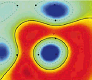
\includegraphics[width=0.15\textwidth]{template/ml_logo}\\
\end{tabular}
%draw a line
\rule{\textwidth}{0.4pt}
%aub: remove this on final submission
%\begin{center}
%DOCUMENT BUILD DATE: \today\\%
%add your status here, e.g. First Draft for Supervizor etc.
%DOCUMENT STATUS: Beta
%\end{center}

%vertical space
\vspace{2.5cm}
\begin{center}
%replace this
  \textbf{\LARGE \trtitle}
\end{center}
\vspace{2cm}

\begin{center}
  \textbf{\trtype} \\
  Fachgebiet Maschinelles Lernen\\
  Prof.\ Dr.\ Klaus-Robert M�ller \\
  Fakult�t IV Elektrotechnik und Informatik \\
  Technische Universit�t Berlin \\[0.5cm]
  submitted by \\
  \textbf{\trauthor}
\end{center}

\vspace{1cm}


\begin{center}
\begin{tabular}{ll}
Instructor:& \trguta\\
& \trgutb\\
\end{tabular}
\end{center}

\vfill

\begin{tabular}{l}
Matrikelnummer:  \trmatrikelnummer \\
Email: \tremail \\
\end{tabular}

\rule{\textwidth}{0.4pt}

\clearpage
%TOC
\tableofcontents
%add list of figures to TOC
\cleardoublepage
\addcontentsline{toc}{chapter}{List of Figures}
\newpage
\listoffigures
%__________________________Main_Content______________________________________________
\newpage
%from now on, numbering should be arabic
\pagenumbering{arabic}
\chapter{Implementation}
\label{implementation}
%#############################################################################################

This chapter explains the implementation of some algorithms that are used in this problem set. It includes: \textit{PCA}, \textit{$\gamma$-index} and \textit{LLE}.

\section{Assignment 1: PCA}
\label{sec:assignment1}

In this assignment the function \textit{pca} has to be implemented, which receives a \textit{d x n} matrix \textit{X} and the number of components \textit{m} as parameters, and returns the principal components as well as the projected data points in a \textit{m x n} matrix \textit{Z}. The principle components should be returned as a \textit{d x d} matrix \textit{U} and a \textit{1 x d} vector \textit{D}. The vector \textit{D} contains the principal values, sorted in descending order ($D_1 \geq D_2 ...$), whereas the matrix \textit{U} contains the principal directions, which corresponds to the sorted principle values.

The implemented function was tested on the test data and passed the test. Following steps are performed in the implementation of the function:
\begin{enumerate}
	\item Substract \textit{X} from its mean.
	\item Calculate the covariance matrix from the zero-mean \textit{X}.
	\item Calculate the eigenvalues and eigenvectors from the covariance matrix.
	\item Sort the eigenvalues and eigenvectors in descending order.
	\item Form the feature vectors by taking only the first \textit{m} eigenvectors.
	\item Project the zero-mean \textit{X} to the feature vectors.
	\item Return the projected data points, principal directions and principal values as \textit{Z}, \textit{U} and \textit{D}.
\end{enumerate}

%######################################################################################
\section{Assignment 2: $\gamma$-Index}
\label{sec:assignment2}

The task in this assignment is to implement the $\gamma$-index which can be used to detect outliers in data set. In their paper, \citeasnoun**{Harmeling2006} formulate the formula to calculate the $\gamma$-index for each data point as follows:
\begin{equation}
	\gamma(x)=\frac{1}{k} \sum_{j=1}^{k} \| x-z_j(x) \|
\end{equation}
where $x$ is a data point, $k$ is the number of nearest neighbours, and $z_1(x),...,z_k(x)$ are the $k$ nearest neighbours of $x$.

The implemented function receives a \textit{d x n} matrix \textit{X} containing the data points and a scalar \textit{k} representing the number of neighbours as parameters. It returns the $\gamma$-index for each data point in a \textit{1 x n} vector \textit{y}.

The function was tested on the test data and passed the test. Following steps are performed in the implementation of the function:
\begin{enumerate}
	\item Implement a helper function \textit{distmat} that calculates the distances from the data points to each other and return the distances as a matrix.
	\item Get the distance matrix using the function \textit{distmat} mentioned above.
	\item Sort the distance matrix in ascending order.
	\item Take only the \textit{k}-nearest data points as neighbours for each data point.
	\item Calculate the mean from the distances of the \textit{k}-nearest neighbours and set it as the $\gamma$-index.
	\item Return the calculated $\gamma$-index as a \textit{1 x d} vector \textit{y}.
	
\end{enumerate}


%######################################################################################
\section{Assignment 3: LLE}
\label{sec:assignment3}

The last task in the implementation part is to implement the \textit{locally linear embedding} method as described by \citeasnoun{Saul2000} in their paper. The implemented \textit{lle} function returns a \textit{m x n} matrix \textit{Y} representing the resulting embedding and takes following parameters as inputs:
\begin{itemize}
	\item A \textit{d x n} matrix \textit{X} containing the data points.
	\item A scalar \textit{m} representing the dimension of the resulting embedding.
	\item A string \textit{n\_rule} determining the method (\textit{'knn'} or \textit{'eps-ball'}) for building the neighbourhood graph.
	\item A scalar \textit{param} used as parameter for the \textit{n\_rule} (\textit{k} or $\epsilon$, respectively).
	\item A scalar \textit{tol} determining the size of the regularization parameter.
\end{itemize}

The implementation is based on the pseudocode described by \citeasnoun{Saul2000} on their website\footnote{http://www.cs.nyu.edu/~roweis/lle/algorithm.html}, which contains of three main parts:
\begin{enumerate}
	\item Find the nearest neighbours of each data point based on \textit{n\_rule}.
	\item Solve for reconstruction weights \textit{W}.
	\item Compute embedding coordinates \textit{Y} using weights \textit{W}.
\end{enumerate}

\chapter{Application}
\label{chap:application}
%#############################################################################################

In this chapter, we are trying to apply the algorithms that are described and implemented in Chapter~\ref{implementation} to various datasets: \textit{usps}, \textit{banana}, \textit{fishbowl}, \textit{swissroll} and \textit{flatroll}.


%#############################################################################################
\section{Assignment 6: \textit{5gaussians} Analysis}
\label{assignment6}

This assignment asks us to apply \textit{PCA} to the \textit{usps} data set and visualizing the results. The \textit{usps} data set consists of 2007 images with the dimension of \textit{16 x 16}. The images are hand-written digits of zero to nine, which can be viewed as classes. Firstly, i separate the data set according to each digit into ten classes and then applied \textit{PCA} to each class. The \textit{PCA} was applied to the original data set and noisy data set.



\begin{figure}[h!]
	\centering
	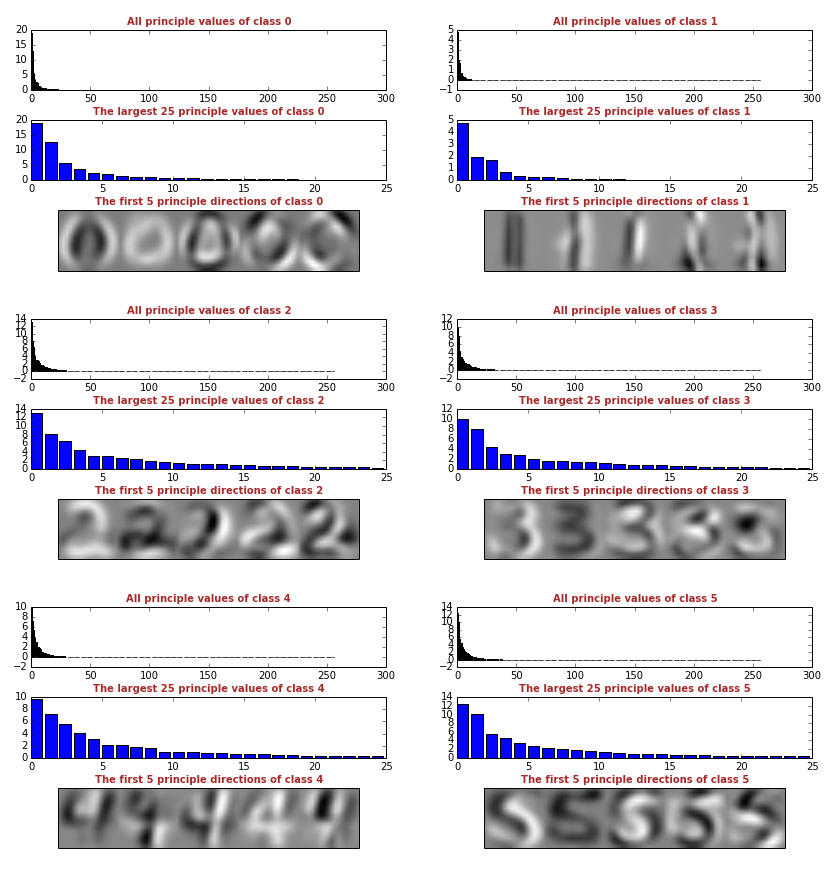
\includegraphics[scale=0.4983]{normalpca_0-5}
	\caption{Principal components of usps original data set for class 0 - 5}
	\label{fig:pcaOriginal05}
\end{figure}


%#############################################################################################
\section{Assignment 7: \textit{2gaussian} Analysis}
\label{assignment7}

In this assignment, the $\gamma$-index method is utilized to detect outliers and applied it to the \textit{banana} data set. The positive class of the data set is used as \textit{inliers}, to which the negative class is added as outliers. The $\gamma$-index is then used to detect outliers with contamination rates of 1\%, 5\%, 10\% and 25\% relative to the positive class. Figure~\ref{fig:bananacomplete} shows the complete original data set, both positive and negative class, whereas Figure~\ref{fig:bananacontaminated} shows the contaminated data set.

\begin{figure}[h!]
	\centering
	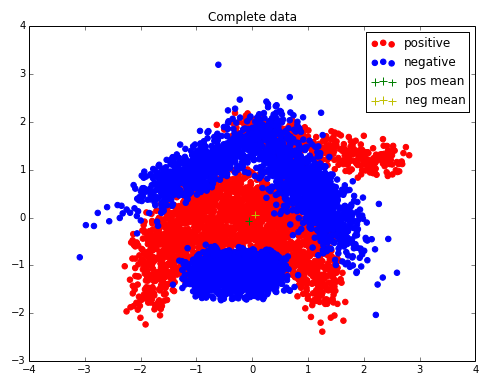
\includegraphics[scale=0.4983]{banana_complete}
	\caption{Both positive and negative of banana data set, including the mean of both classes}
	\label{fig:bananacomplete}
\end{figure}

\begin{figure}[h!]
	\centering
	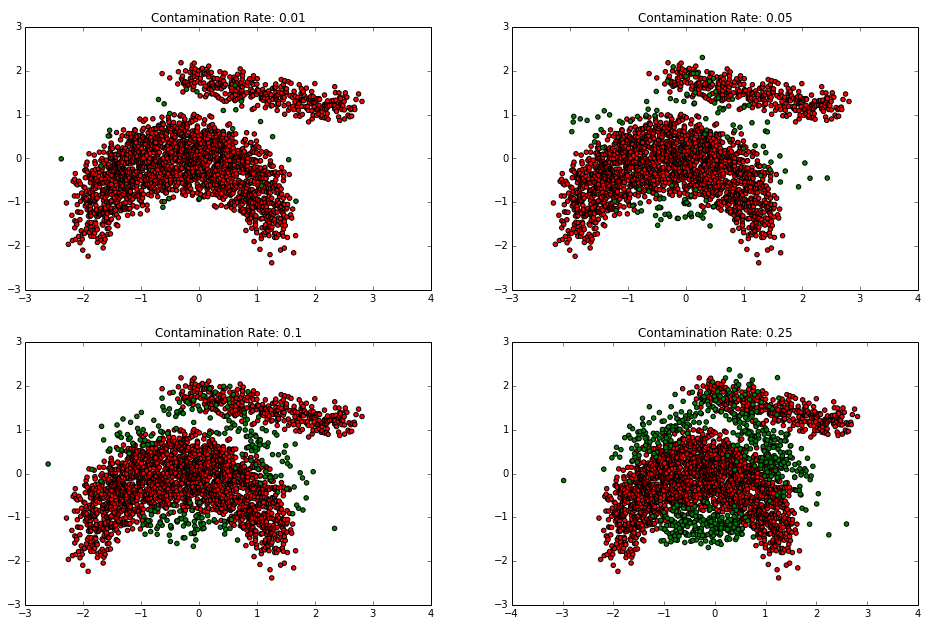
\includegraphics[scale=0.4983]{banana_contaminated}
	\caption{Contaminated banana data set with contamination rate of 1\%, 5\%, 10\% and 25\%}
	\label{fig:bananacontaminated}
\end{figure}

There are three methods that should be used to detect the outliers: (a) the $\gamma$-index with $k=3$, (b) the $\gamma$-index with $k=10$ and (c) the distance to the mean for each data point. All of the methods are then applied to the four contamination rates mentioned above. After that, the \textit{AUC} (area under the \textit{ROC}) should be calculated. Figure~\ref{fig:gammaboxplots} shows the boxplots that visualize the distribution of the \textit{AUC} values.

\begin{figure}[h!]
	\centering
	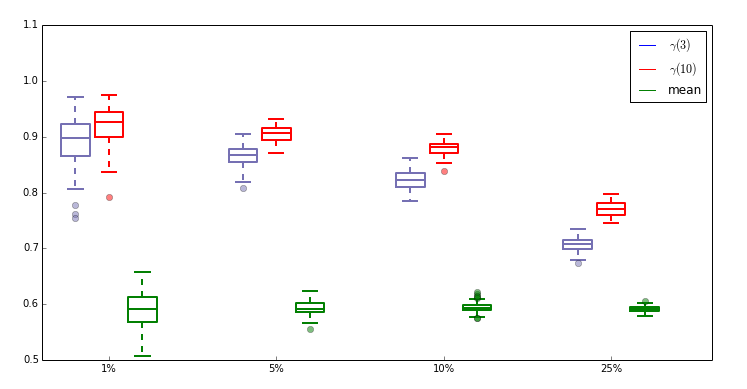
\includegraphics[scale=0.5583]{gamma_boxplots}
	\caption{Boxplots visualizing the distribution of the \textit{AUC} values}
	\label{fig:gammaboxplots}
\end{figure}

The boxplots show that the method using the distance to the mean for each data point performed quite bad, while both of the $\gamma$-index methods performed very well, especially for the data set with lower contamination rates. The $\gamma$-index with $k=10$ performed slightly better than the $\gamma$-index with $k=3$.


%#############################################################################################

\section{Assignment 8: \textit{USPS} Analysis}
\label{assignment8}

In the last assignment of this problem set, \textit{LLE} has to be applied to noisy \textit{flatroll} data set. Two gaussian noise were added to the data set, with variance 0.2 and 1.8, respectively. After that, both noisy data sets should be unrolled using \textit{knn} with a good value of \textit{k} and a value which is obviously too large. Figure~\ref{fig:llenoisy} depicts the two noisy images and their resulting embedding. It can be obtained that the noisy data set with big variance(1.8) is not very good unrolled.

\begin{figure}[h!]
	\centering
	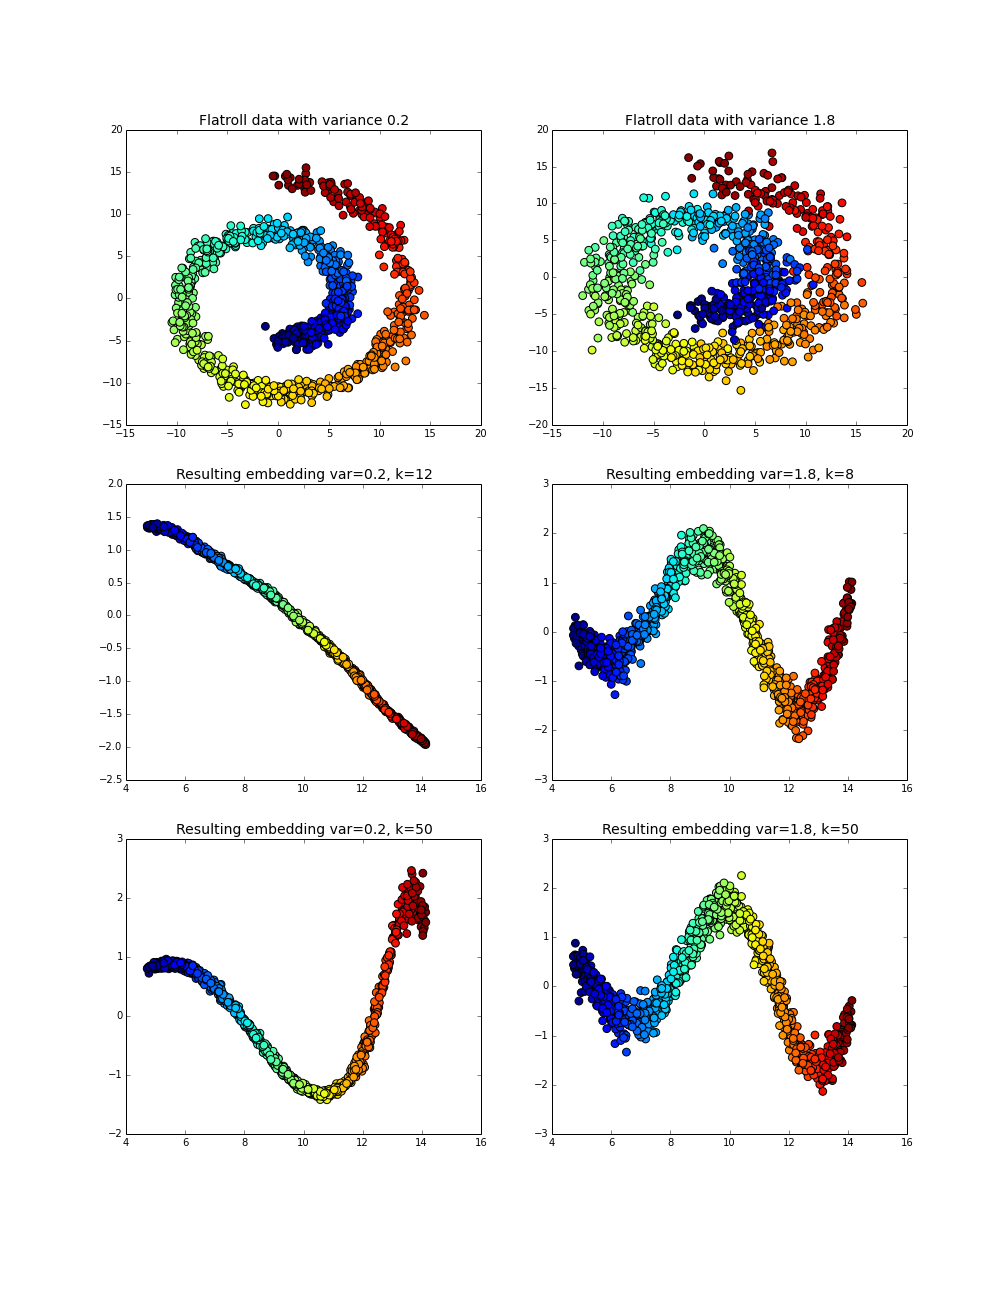
\includegraphics[scale=0.4983]{lle_noise}
	\caption{Visualization of two noisy \textit{flatroll} data set and their resulting embedding}
	\label{fig:llenoisy}
\end{figure}


%__________________________End_of_Thesis______________________________________________
\cleardoublepage
\addcontentsline{toc}{chapter}{Bibliography}
%harvard citations style, please uncomment harvard package in the usepackage area
\bibliographystyle{agsm}
%remove the following line when using harvard style citation
%\bibliographystyle{plain}
%specify bibtex file here
\bibliography{input/mybib}

\end{document}
